\begin{center}
	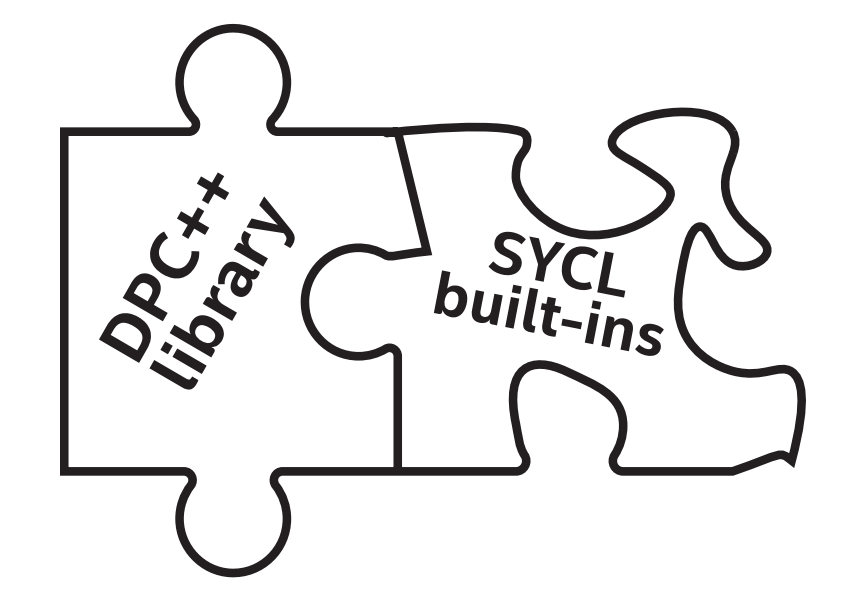
\includegraphics[width=0.5\textwidth]{content/chapter-18/images/1}
\end{center}

We have spent the entire book promoting the art of writing our own code. Now we finally acknowledge that some great programmers have already written code that we can just use. Libraries are the best way to get our work done. This is not a case of being lazy—it is a case of having better things to do than reinvent the work of others. This is a puzzle piece worth having.\par

The open source DPC++ project includes some libraries. These libraries can help us continue to use libstdc++, libc++, and MSVC library functions even within our kernel code. The libraries are included as part of DPC++ and the oneAPI products from Intel. These libraries are not tied to the DPC++ compiler so they can be used with any SYCL compiler.\par

The DPC++ library provides an alternative for programmers who create heterogeneous applications and solutions. Its APIs are based on familiar standards—C++ STL, Parallel STL (PSTL), and SYCL—to provide highproductivity APIs to programmers. This can minimize programming effort across CPUs, GPUs, and FPGAs while leading to high-performance parallel applications that are portable.\par

The SYCL standard defines a rich set of built-in functions that provide functionality, for host and device code, worth considering as well. DPC++ and many SYCL implementations implement key math built-ins with math libraries.\par

The libraries and built-ins discussed within this chapter are compiler agnostic. In other words, they are equally applicable to DPC++ compilers or SYCL compilers. The fpga\_device\_policy class is a DPC++ feature for FPGA support.\par

Since there is overlap in naming and functionality, this chapter will start with a brief introduction to the SYCL built-in functions.\par



















